% This is "sig-alternate.tex" V2.1 April 2013
% This file should be compiled with V2.5 of "sig-alternate.cls" May 2012
%
% This example file demonstrates the use of the 'sig-alternate.cls'
% V2.5 LaTeX2e document class file. It is for those submitting
% articles to ACM Conference Proceedings WHO DO NOT WISH TO
% STRICTLY ADHERE TO THE SIGS (PUBS-BOARD-ENDORSED) STYLE.
% The 'sig-alternate.cls' file will produce a similar-looking,
% albeit, 'tighter' paper resulting in, invariably, fewer pages.
%
% ----------------------------------------------------------------------------------------------------------------
% This .tex file (and associated .cls V2.5) produces:
%       1) The Permission Statement
%       2) The Conference (location) Info information
%       3) The Copyright Line with ACM data
%       4) NO page numbers
%
% as against the acm_proc_article-sp.cls file which
% DOES NOT produce 1) thru' 3) above.
%
% Using 'sig-alternate.cls' you have control, however, from within
% the source .tex file, over both the CopyrightYear
% (defaulted to 200X) and the ACM Copyright Data
% (defaulted to X-XXXXX-XX-X/XX/XX).
% e.g.
% \CopyrightYear{2007} will cause 2007 to appear in the copyright line.
% \crdata{0-12345-67-8/90/12} will cause 0-12345-67-8/90/12 to appear in the copyright line.
%
% ---------------------------------------------------------------------------------------------------------------
% This .tex source is an example which *does* use
% the .bib file (from which the .bbl file % is produced).
% REMEMBER HOWEVER: After having produced the .bbl file,
% and prior to final submission, you *NEED* to 'insert'
% your .bbl file into your source .tex file so as to provide
% ONE 'self-contained' source file.
%
% ================= IF YOU HAVE QUESTIONS =======================
% Questions regarding the SIGS styles, SIGS policies and
% procedures, Conferences etc. should be sent to
% Adrienne Griscti (griscti@acm.org)
%
% Technical questions _only_ to
% Gerald Murray (murray@hq.acm.org)
% ===============================================================
%
% For tracking purposes - this is V2.0 - May 2012

\documentclass{sig-alternate-05-2015}
\usepackage{graphicx}
\usepackage{algorithm2e}
\usepackage{multirow}
\begin{document}


\title{Distributed Neural Networks: A Parallel Approach}
\numberofauthors{2} %  in this sample file, there are a *total*
% of EIGHT authors. SIX appear on the 'first-page' (for formatting
% reasons) and the remaining two appear in the \additionalauthors section.
%
\author{
%
% The command \alignauthor (no curly braces needed) should
% precede each author name, affiliation/snail-mail address and
% e-mail address. Additionally, tag each line of
% affiliation/address with \affaddr, and tag the
% e-mail address with \email.
%
% 1st. author
\alignauthor
Tasneem Alowaisheq\\
       \affaddr{Indiana University}\\
       \affaddr{107 S Indiana Ave}\\
       \affaddr{Bloomington, USA}\\
       \email{talowais@indiana.edu}
% 2nd. author
\alignauthor
Devendra Singh Dhami\\
       \affaddr{Indiana University}\\
       \affaddr{107 S Indiana Ave}\\
       \affaddr{Bloomington, USA}\\
       \email{ddhami@indiana.edu}
}

\maketitle
\begin{abstract}
This paper provides an insight into our work in designing distributed neural networks. In this paper we are implementing a parallel mini-batch back propagation algorithm using Hadoop framework. Our results show that the parallel algorithm converges faster than the sequential algorithm, remaining comparable in the accuracy achieved.
\end{abstract}


%
% The code below should be generated by the tool at
% http://dl.acm.org/ccs.cfm
% Please copy and paste the code instead of the example below. 
%

\ccsdesc[500]{Distributed neural network~Parallelism}
\ccsdesc[300]{Distributed systems~Hadoop}
\ccsdesc{Distributed systems~Harp}
%
% End generated code
%

%
%  Use this command to print the description
%
\printccsdesc


\section{Introduction - Motivation}
Neural networks are models that were motivated by the structure of the human brain and were built to mimic its functioning. It has several layers of interconnected neurons that form an artificial network, as shown in figure \ref{NN}, and is typically defined by:
\begin{figure}[h]
\centering
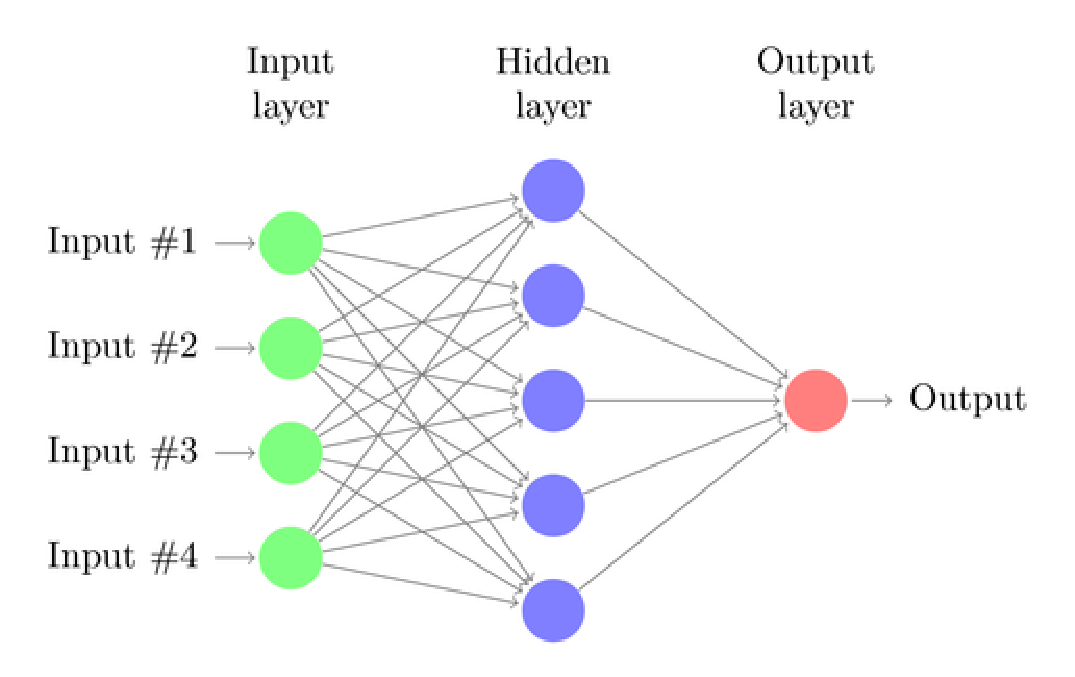
\includegraphics[width=4cm]{img/neural-network}
\caption{An example neural net}
\label{NN}
\end{figure}
\begin{enumerate}
\item Weights: This refers to the weight that connects between the different neurons in the layers.
\item Learning: This refers to the process of learning (by back propagating the error) and calculating the derivatives for updating the weights.
\item Activation Function: This refers to the function that converts the sum of a neuron's weighted input to the output.
\end{enumerate}
Thus, the neural networks can be considered as directed graphs with each layer consisting of a set of neurons. The training data is passed in the input layer; the hidden layer learns an abstraction of the input data and finally we get the output from the output layer.
Creating a distributed neural network can be beneficial in several cases:
\begin{enumerate}
\item The data is large and cannot be handled by one process.
\item For complex structures the size of a layer becomes too large for one process to handle.
\end{enumerate}
Due to the above defined reasons, having a parallel version of the neural network model becomes an important problem which is well studied in the machine learning and distributed systems community. Next we discuss the related work in section \ref{RW} and give a problem definition in section \ref{Problem Definition}. Section \ref{PM} defines our proposed method and section \ref{E} and section \ref{C} present the experiments and conclusion respectively.

\section{Related Work} \label{RW}
In late 90s and early 2000s the neural network architecture consisted of relatively small number of layers and units per layer. This limitation was mainly due to the relatively slow machines which made the training of large networks inefficient. For the MNIST dataset, methods such as SVMs were able to outperform neural networks. Ciresan et al \cite{ciresan2010deep} explains how these difficulties effected the parallelization of the neural network and how these can be overcome by training the model on graphics cards. They showed that the advancements in the computational resources facilitate training larger neural networks efficiently thereby helping neural networks to achieve high accuracy on the MNIST data. They showed that large networks with many parameters can be trained to achieve error below 1\% in less epochs and thus less time.
LeCunn et al \cite{lecun2012efficient} present some tricks to perform efficient backpropagation. Some of the tricks briefly are: 
\begin{enumerate}
\item Incremental stochastic learning performs better than batch learning
\item Shuffling the data after each epoch
\item Input normalization
\item Choosing a better sigmoidal function
\end{enumerate}
They present the advantages and disadvantages of all these tricks and at the end give a few steps to be followed to increase the accuracy and efficiency of the neural network models.
Dean et al \cite{dean2012large} create a distributed framework to train large sized deep networks on
thousands of CPU cores and give an efficient SGD algorithm for these networks. They call this framework \textit{DistBelief} within which they implement two novel methods:\\
\begin{enumerate}
\item Downpour SGD, an asynchronous SGD algorithm, and
\item Sandblaster L-BFGS that uses both data and model parallelism. 
\end{enumerate}
They show that this distributed approach can result in speedup of the training time of large models using clusters of machines which take very less time when compared to training on GPUs. They also show that they could train models larger than any other models existing during that time. They trained a neural network of more than 1 billion parameters and showed that this network achieves better performance compared to the best performing deep neural net model on the ImageNet dataset.

\section{Problem Definition} \label{Problem Definition} 
In this project our main goal is to design a distributed neural network to get a classification performance with less training time comparable to the sequential neural network.
This problem can be approached in two ways. 
\begin{enumerate}
\item Distributing the network structure horizontally i.e. distributing the neurons in each layer to separate processes. The motivation for this approach is that for complex structures the size of a layer becomes too large for one process to handle.
\item Distributing the dataset to separate processes while keeping the structure of the neural network intact. The motivation for this approach is that the dimensions of the data might be large and thus cannot be handled by one process.
\end{enumerate}  

\section{Proposed Method} \label{PM}
Our aim is to parallelize the training of the neural network by implementing a parallel mini-batch backpropagation algorithm. We are to trying to handle the second case mentioned in section \ref{Problem Definition}. The parallelization can be done in two ways:
\begin{enumerate}
\item Model/Parameter averaging
\item Derivative averaging
\end{enumerate}
As suggested by \cite{su2015experiments}, model averaging works better in practice, especially when using a large mini-batch size. Our method is based on the parallelization using model averaging manner. \\
The method used for training the neural network is mini-batch gradient descent.
\newdef{definition}{Definition}
\begin{definition}
In mini batch gradient descent, the gradient is computed against more than one training example and less than for the complete training examples i.e. it's in between stochastic and batch gradient descent.
\end{definition}
When we have large data, using a single process will slow down the training of the model considerably. To speed this process up one can randomly sample mini batches with replacement from the training data and distribute the learning over different processes. Each process will train on its local mini-batch data that consists of the feature vectors \textbf{X} and its corresponding targets \textbf{Y}, and the local weights will be updated accordingly. The weights are a vector of matrices where each matrix holds the weight connections from one layer to the next. These weight matrices are flattened and concatenated to get the final representation of the weights to be distributed.\\
These local weights, across all the processes, will then be combined by using \
\textit{Allreduce}, which is called for every five epochs to ensure that the weights are updated across tasks more frequently, and then averaged to obtain the final weights. These weights are the final model used for prediction on the test data. The prediction is not an expensive operation and thus can be handled by the master process. This process is repeated on ten random splits of training and testing data to ensure that we have a good estimate of the generalization error. This process can be shown in figure \ref{meth} where every batch represents a mini batch where the intersection of each mini batch is not $\phi$. 

\begin{figure}[h]
\centering
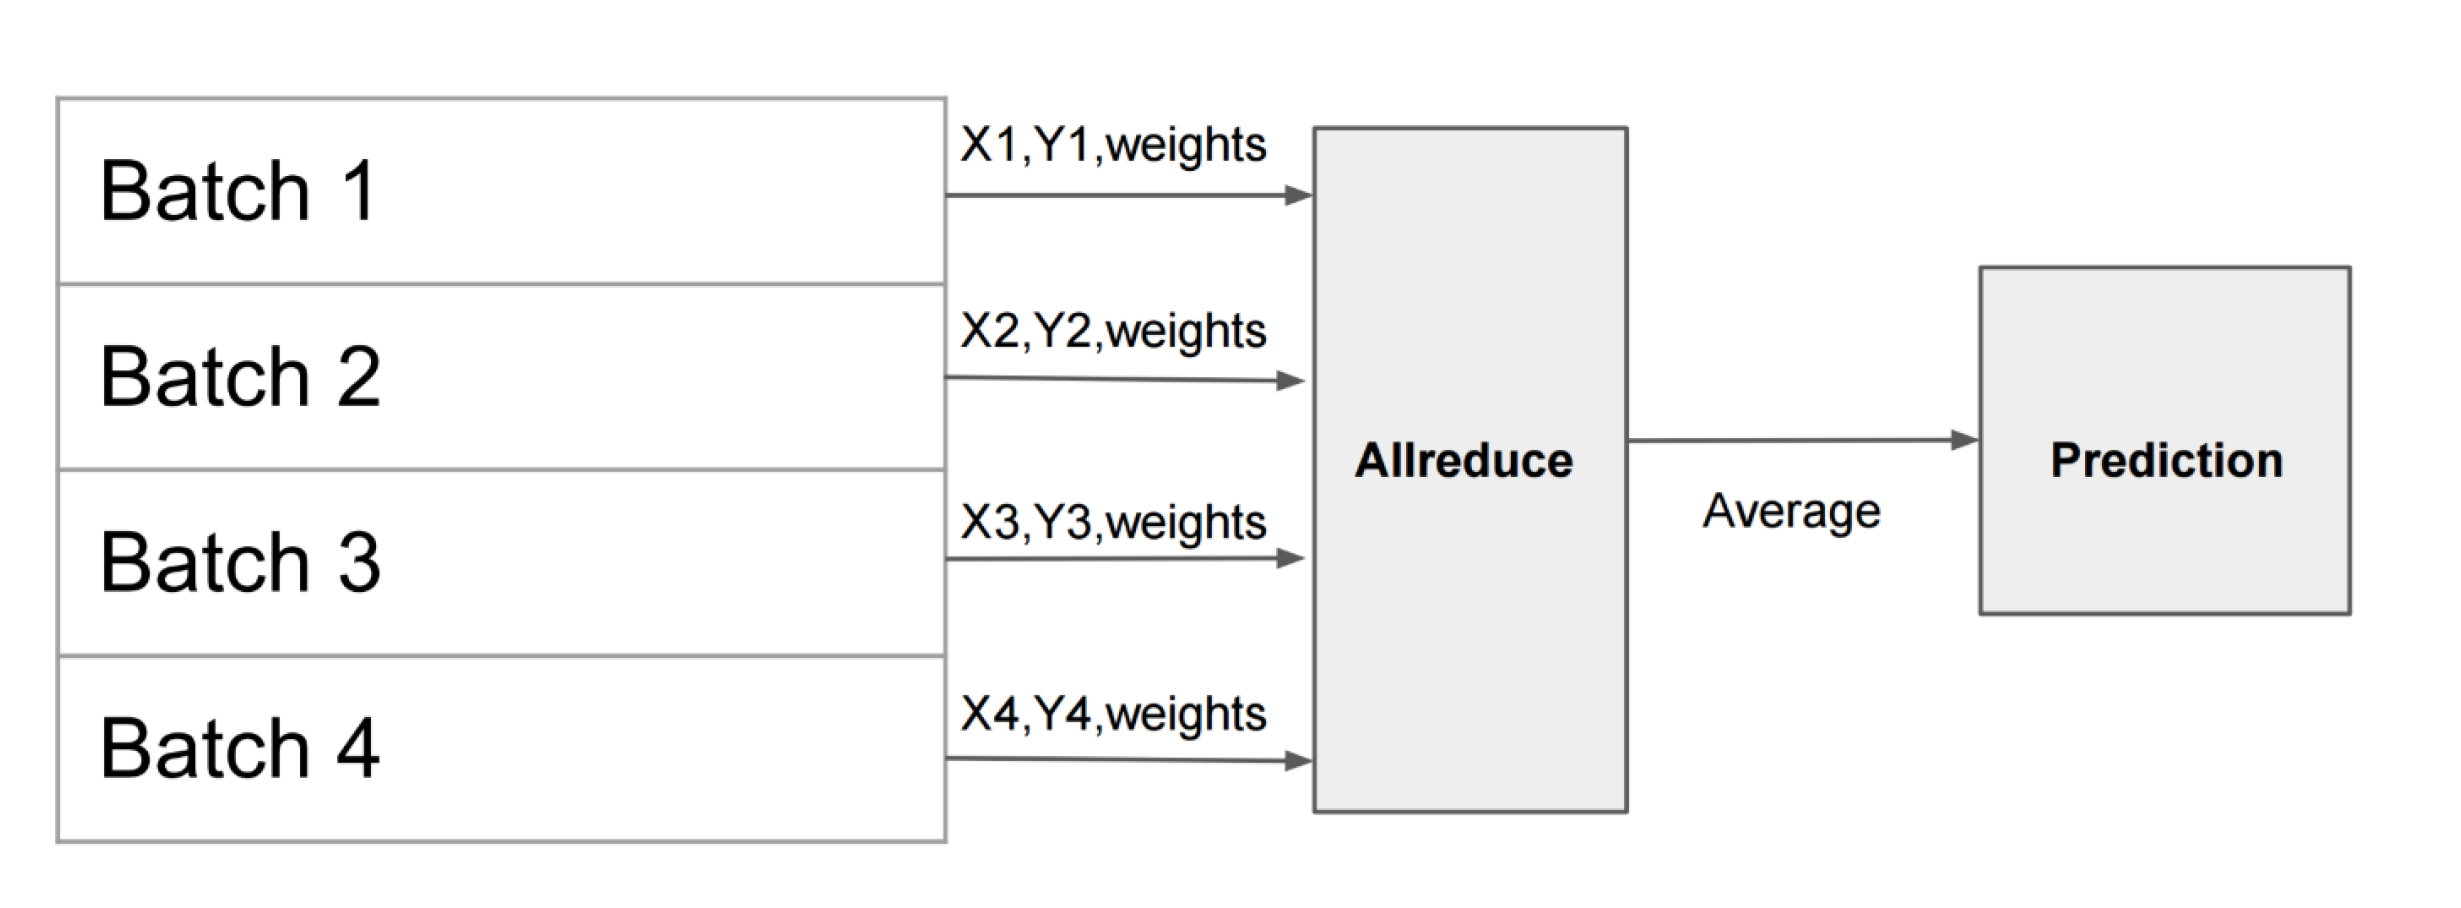
\includegraphics[width=\columnwidth]{img/method}
\caption{The proposed method.}
\label{meth}
\end{figure}

Our proposed algorithm is shown below.

\begin{algorithm}[h]
 \KwData{The input data and corresponding labels}
 \KwResult{List of accuracies across N splits }
 \For{the number of splits, N}{
  Divide the data randomly into training and testing\;
  Initialize the weights\;
 \For{(number of iterations / 5)}{
  Randomly sample the mini batch from training\;
  Train for 5 epochs to update the weights locally\;
  Allreduce\;
  Average the models\;
 }
 \If{master}{
 Predict on test and report accuracy;
 }
 }
 \caption{Parallel neural network}
\end{algorithm}
We make use of mini-batch gradient descent here as it has been shown to be effective for the optimization of the objective function \cite{seide2011conversational}. The size of mini batch should be as large as possible for effective training.
A simplied algorithm for illustrating mini-batch gradient descent is shown in algorithm \ref{mbgd}.\\ \\
\begin{algorithm}[h]
 \KwData{The training data}
 \KwResult{Optimized parameters}
 \For{number of epochs}{
  shuffle the data\;
  \For{every mini batch}{
    Update the parameters;
    }
   }
   \caption{Mini batch gradient descent}
   \label{mbgd}
\end{algorithm}
 
%\begin{table}
%\centering
%\caption{Frequency of Special Characters}
%\begin{tabular}{|c|c|l|} \hline
%Non-English or Math&Frequency&Comments\\ \hline
%\O & 1 in 1,000& For Swedish names\\ \hline
%$\pi$ & 1 in 5& Common in math\\ \hline
%\$ & 4 in 5 & Used in business\\ \hline
%$\Psi^2_1$ & 1 in 40,000& Unexplained usage\\
%\hline\end{tabular}
%\end{table}

%To set a wider table, which takes up the whole width of
%the page's live area, use the environment
%\textbf{table*} to enclose the table's contents and
%the table caption.  As with a single-column table, this wide
%table will ``float" to a location deemed more desirable.
%Immediately following this sentence is the point at which
%Table 2 is included in the input file; again, it is
%instructive to compare the placement of the
%table here with the table in the printed dvi
%output of this document.


%\begin{table*}
%\centering
%\caption{Some Typical Commands}
%\begin{tabular}{|c|c|l|} \hline
%Command&A Number&Comments\\ \hline
%\texttt{{\char'134}alignauthor} & 100& Author alignment\\ \hline
%\texttt{{\char'134}numberofauthors}& 200& Author enumeration\\ \hline
%\texttt{{\char'134}table}& 300 & For tables\\ \hline
%\texttt{{\char'134}table*}& 400& For wider tables\\ \hline\end{tabular}
%\end{table*}
% end the environment with {table*}, NOTE not {table}!



\section{Experiments} \label{E}
We report the results for ten randomly sampled training and test splits for both the sequential code and the parallel code. The task is a digit classification task that consists of the grayscale pixels intensities of the image as a feature vector and the target is a vector of size 10 where each element is one for the corresponding digit and zero elsewhere. The data set consists of 5000 examples. For fair comparison, we made sure that the splits across different experiments are the same and random weight initialization is the same by setting the seed to the split number. The weights are initialized from a uniform distribution in range [0,1]. For generating the splits, 70\% is used for training purposes and 30\% for testing. For the following experiments, the mini batch size is 90\% of the training data.\\
We utilized the open source sequential code from \cite{dvincentNN} to implement our parallel method. We changed the sequential code to a mini-batch version to use it as a baseline for comparison. Also we changed the weight initialization for the sequential code from normal to uniform distribution for the sake of fair comparison. The parameters for both methods are:
\begin{enumerate}
\item regularization parameter, $\lambda$ = 0.6987.
\item learning rate, learned using line search.
\end{enumerate}

We run the sequential code on the local machine and the parallel version on the Juliet cluster for 2, 4 and 8 map tasks using two nodes. Each experiment yields ten accuracies we average them to get the final accuracy. The average accuracies for both are presented in table \ref{res} below.

\begin{table} [h]
\centering
\caption{Average accuracies for sequential and parallel NN} 
\begin{tabular}{|c|c|c|} \hline
Number of Epochs&Sequential&Parallel\\ \hline
100&80.67\%&84.06\%\\ \hline
200&86.89\%&87.28\%\\ \hline
250&88.63\%&86.45\%\\ \hline
500&89.9\%&88.93\%\\ \hline
\end{tabular}
\label{res}
\end{table}
		
Note that we present only one accuracy for the parallel algorithm since the different number of mappers yield the same accuracy which is expected as the random sampling is fixed across experiments. 

As figure \ref{acc_NN} shows, when having enough number of epochs both the parallel and the sequential methods yield about the same accuracy. 
\begin{figure}[h!]
\centering
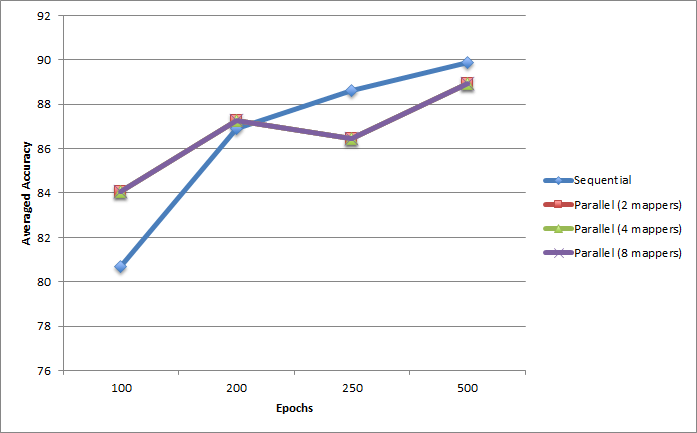
\includegraphics[width=\columnwidth]{img/accuracies}
\caption{Average accuracies for the neural network.}
\label{acc_NN}
\end{figure}

The convergence times for the sequential and parallel neural network is shown in table \ref{mapper_res}.
\begin{table} [h!]
\centering
\caption{Average convergance time for sequential and parallel NN} 
\begin{tabular}{|c|c|c|c|c|c|} \hline
Epochs&Sequential&Parallel(2)&Parallel(4)&Parallel(8)\\ \hline
100&244 sec&211 sec&209 sec&217 sec\\ \hline
200&494 sec&337 sec&318 sec&345 sec \\ \hline
250&622 sec&406 sec&398 sec&431 sec \\ \hline
500&1225 sec&790 sec&746 sec&807 sec \\ \hline
\end{tabular}
\label{mapper_res}
\end{table}

In terms of convergence, parallel methods converges faster than the sequential one as shown in figure \ref{time_NN}, it seems that the gap in convergence have an exponential property in terms of the number of epochs. 
\begin{figure}[h!]
\centering
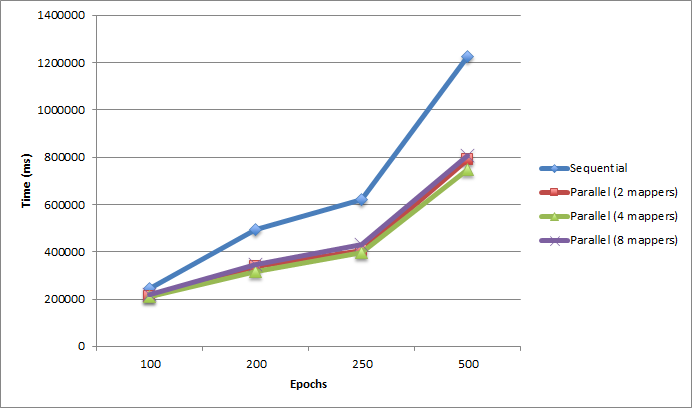
\includegraphics[width=\columnwidth]{img/time}
\caption{Time taken for convergence by the neural network.}
\label{time_NN}
\end{figure}


Figure \ref{map_NN} show the time when using different number of mappers. All experiments yielded about the same time for different epochs. 
\begin{figure}[h!]
\centering
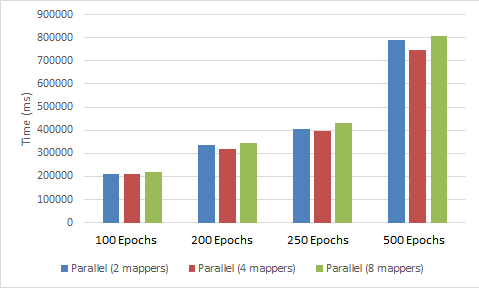
\includegraphics[width=\columnwidth]{img/time_map}
\caption{Time taken for convergence by the parallel neural network for different number of mappers.}
\label{map_NN}
\end{figure}

We needed to change some of the default Hadoop settings in order for our method to work:  For experiments with a large number of epochs some jobs failed due to exceeding the task timeout. We increased the \textit{mapred.task.timeout} for the job configuration in the \textit{MapCollective}. Also when increasing the number of mappers some jobs failed so we changed the memory settings in the \textit{mapred-site.xml} and \textit{yarn-site.xml}.

\section{Conclusions} \label{C}
In this paper we presented a parallel implementation for the mini-batch neural network. We demonstrated our method on a digit classification task. Our results show that the parallel version is comparable to the sequential one in terms of accuracy and converged significantly faster than the sequential method.

%
% The following two commands are all you need in the
% initial runs of your .tex file to
% produce the bibliography for the citations in your paper.

\bibliographystyle{abbrv}
\bibliography{sigproc} 
\appendix
%Appendix A

\section{Acknowledgments}
We would like to thank Bo Peng for his feedback on our method and Raksha Kumaraswamy for helping us in setting up the juliet cluster.\\
\end{document}